\newpage
\section{Movilidad en Mininet-Wifi}
Unos de los aspectos más interesantes de este emulador es la posibilidad que tienen los nodos de la topología de ser "moviles". Mininet-Wifi hace uso de del modulo de kernel llamado \textit{mac80211\_hwsim} que crea un medio virtual para todos los nodos inalámbricos. Esto significa que todos los nodos están internamente en rango uno de otros y pueden ser descubiertos en un barrido wireless por sus interfaces inalámbricas virtuales. \newline
\newline
Para dotar de sentido a la topología, Mininet-Wifi simula sus posiciones y rangos para cada nodo y gestiona quien está en rango para asociarse a un punto de acceso o quien puede intercambiar paquetes con otro nodo. Esto lo hace revocando las asociaciones entre estos nodos, por así decirlo trabaja como Hypervisor del medio Wireless para que este medio aunque sea un medio virtual se asemeje lo más posible a un entorno real.
\begin{figure}[!htb]
  \centering
    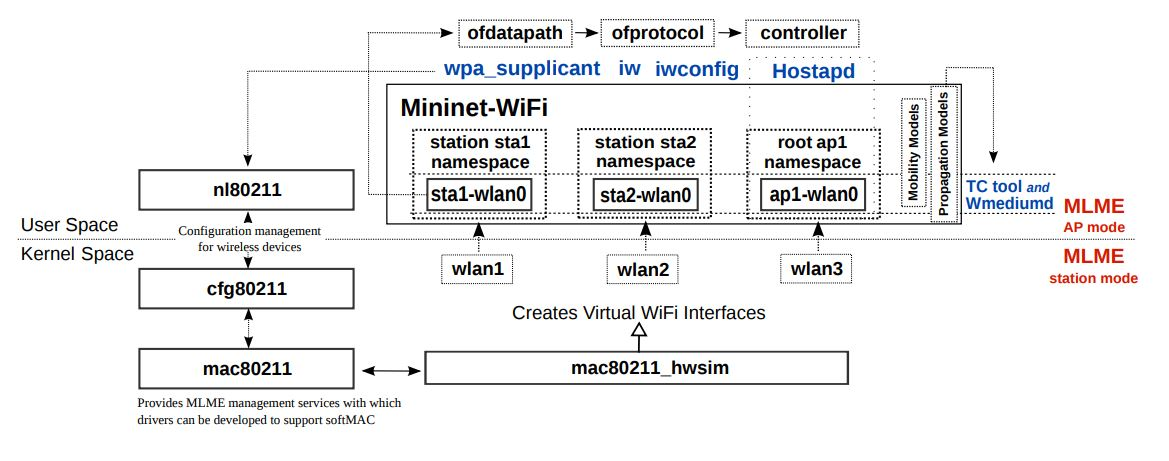
\includegraphics[width=0.9\linewidth]{./img/movi/1.JPG}
    \caption{Operativa Mininet-Wifi.}
  \label{fig:yo}
\end{figure}
\subsection{Tipos de movilidad}
Como hemos dicho Mininet-Wifi simula la posición de cada nodo en la red (Estaciones wifi y puntos de acceso), por lo que tiene su posición en un espacio tridimensional parametrizada, con esto Mininet-Wifi es capaz de simular la movilidad de sus nodos en un espacio virtual. Mininet-Wifi tiene distintas herramientas para implementar la movilidad en una emulación:
\begin{itemize}
    \item La primera de ellas es con un método llamado \textbf{setPosition()} de esta manera podremos indicarle dinámicamente a un nodo las posiciones que queremos que tome (X,Y,Z). Visto de esta manera estaríamos teletransportando a un nodo a unas coordenadas concretas, pero con una correcta gestión del tiempo podremos simular un buen modelo de movilidad para un nodo.Al fin y al cabo, los distintos modelos de movilidad que se van a exponer hacen uso de este método, lo importante es la gestión que hay entorno a él. Ejemplo: \textit{py sta1.setPosition('20,150,0')}
    \item La segunda herramienta que nos provee Mininet-Wifi es una serie de métodos para indicar el punto inicial y final para un nodo, indicando un tiempo inicial y un tiempo final. Pdremos hacer uso de estos metodos via la API de Python que tienen dispuesta. Por ejemplo, la movilidad para una estación wifi, con un criterio de asociación a los puntos de acceso SSF (Strongest Signal First)
    \begin{minted}[]{python}
        info("*** Configurando Movilidad (sta1)\n")
        net.startMobility(time = 0, AC='ssf')
        
        # Indicamos x0, x1, Tinit, Tfin
        net.mobility(sta1, 'start', time = 20, position='1,50,0')
        net.mobility(sta1, 'stop', time = 79, position='159,50,0')
        
        net.stopMobility(time=200)
        
    \end{minted}
    \newpage
    \item Por último, Mininet-Wifi nos brinda modelos de movilidad ya predefinidos.
        \begin{itemize}
            \item RandomWalk
            \item TruncatedLevyWalk
            \item RandomDirection
            \item RandomWayPoint
            \item GaussMarkov
            \item ReferencePoint 
            \item TimeVariantCommunity
        \end{itemize}
\end{itemize}
Estos modelos se caracterizan por tomas de decisiones de movimiento equiprobables, hay distintos tipos de RandomWalks en función del numero de dimensiones, velocidad, intervalo de tiempo de tomas de decisiones. También hay modelos que aplican el Random walk entorno a un punto de referencia, o la posición de uno de sus nodos de la topología
\begin{figure}[!htb]
  \centering
    
\includegraphics[width=\linewidth]{./img/movi/2.png}
    \caption{RandomWalk en dos dimensiones.}
  \label{fig:yo}
\end{figure}
\newpage
\begin{figure}[!htb]
  \centering
    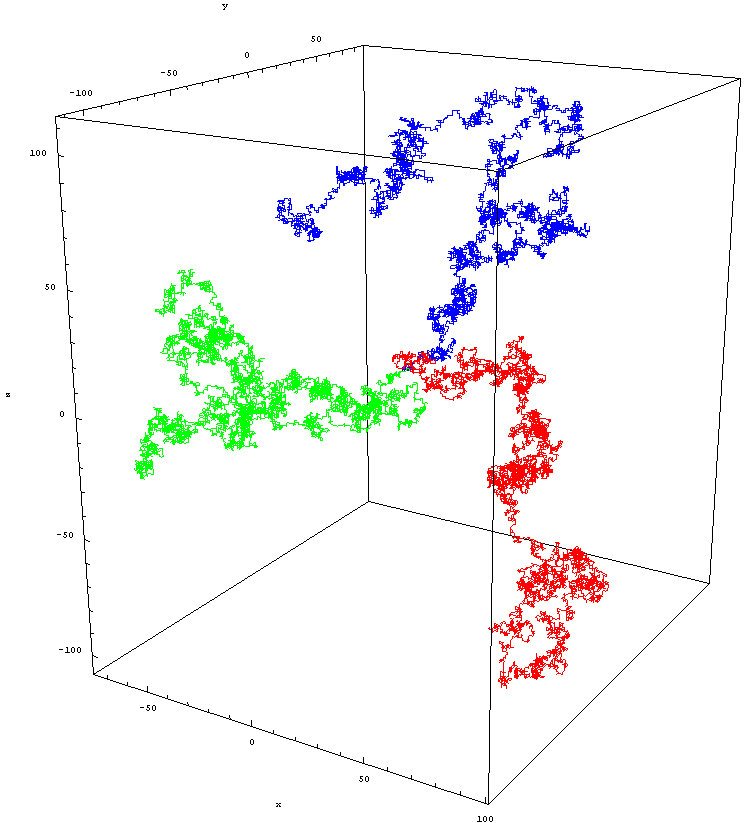
\includegraphics[width=0.9\linewidth]{./img/movi/3.png}
    \caption{RandomWalk en tres dimensiones.}
  \label{fig:yo}
\end{figure}
Nosotros haremos uso mayoritariamente de la segunda herramienta que nos provee Mininet-Wifi. Nota: Hay que hacer pull-request de los cambios hecho en la gestión de los Threads para gestión la movilidad vía CLI
\newpage

